\section{Approach Overview}
\label{overview:sec}

\subsection{Important Concepts}
\label{concepts:sec}

\begin{figure}[t]
	\centering
	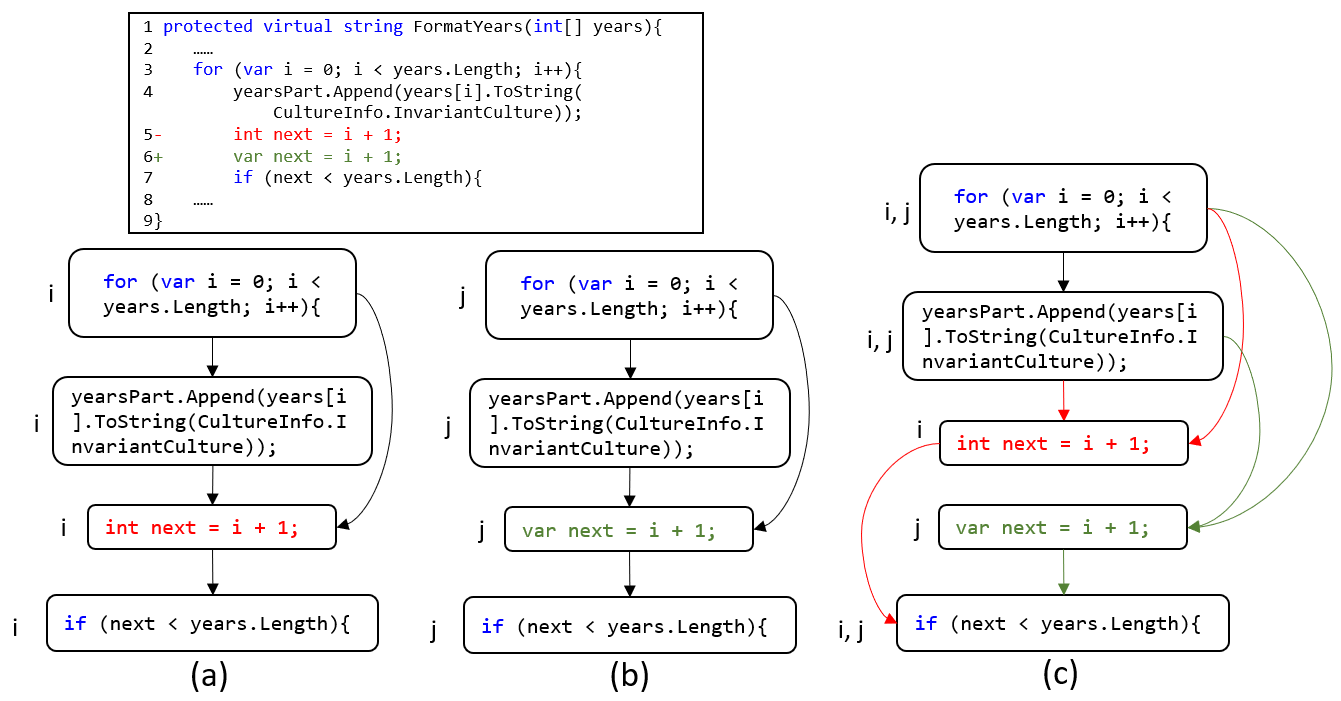
\includegraphics[width=3.5in]{figures/multi-version-graph-3.png} %5.3
	\vspace{-18pt}
	\caption{Multi-Version Program Dependence Graph}
	\label{fig:multi-version-pdg}
\end{figure}

\begin{figure*}[t]
	\centering
 	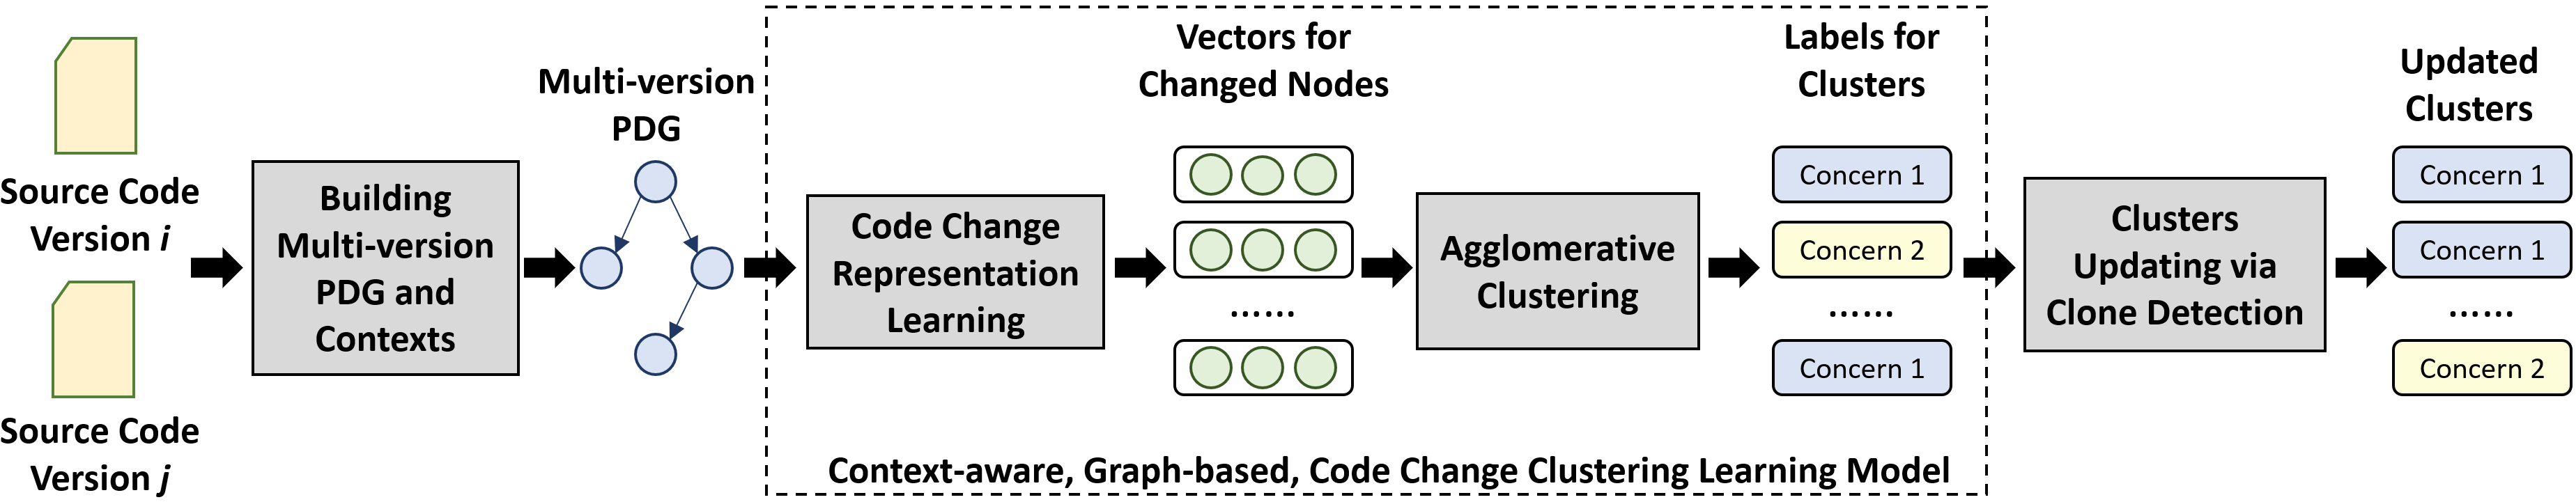
\includegraphics[width=6in]{figures/overview-3.png}
	\vspace{-6pt}
	\caption{{\tool}: Architecture Overview}
	\label{fig:overview}
\end{figure*}

Let us first define some important concepts used in {\tool}.

%First, we formally define the PDG, multi-version PDG, changed/unchanged statements, and context to conduct our approach's overview. Within these definitions, We re-use the definition of program dependency graph and multi-version program dependency graph from Partachi et al.'s research \cite{flexeme-fse20}.

\begin{Definition}[Program Dependence Graph]
The \textbf{program dependency graph (PDG)}~\cite{pdg} is a directed
graph with a set $N$ of nodes and a set $E$ of edges such that each
node $n \in N$ represents a program statement or a conditional
expression; each edge $e \in E$ represents the data or control flow
among the statements.
\end{Definition}

%s.t. each node 𝑛 ∈ 𝑁 is annotated with either a program statement or a
%conditional expression; each edge 𝑒 ∈ 𝐸 has an optional annotation
%representing the name or the data that flows along it, and a kind that
%describes the relationship type: data or control.

Figure~\ref{fig:multi-version-pdg} shows the code change in a commit
in which the statement \code{int next = i + 1;} is replaced by
\code{var next = i + 1;}. Figure~\ref{fig:multi-version-pdg} (a) and
(b) display the PDGs of the method \code{FormatYear} before and after
the change. All the nodes of the PDG before the change are marked with
$i$, and those of the PDG after the change are marked with $j$.

%As shown in figure \ref{fig:multi-version-pdg}, the graph with all nodes labeled $i$, and the graph with all nodes labeled with $j$ is the PDG for the version $i$ and version $j$ of the method $FormatYear$. After having these two PDGs, we can define the multi-version program dependency graph. $\delta$-PDG$^{i,j}$

\begin{Definition}[Multi-version Program Dependence Graph] ({\bf $\delta$-PDG}).
A {\mvpdg}~\cite{flexeme-fse20} is a directed graph generated from the
disjoint union of all nodes and edges in the PDGs at versions $i$
and~$j$.
%
%  The \textbf{multi-version program dependency graph (Multi-version PDG$^{i,j}$)} is a directed graph that generated from the disjoint union of all nodes and edges between the version $i$ and version $j$. $\delta-PDG^{i,i}$ is the PDG at the version $i$.
\end{Definition}

Figure~\ref{fig:multi-version-pdg}(c) displays the multi-version
PDG$^{i,j}$ ({\mvpdg}) that are built from the two
versions $i$ and $j$ of the method \code{FormatYear} before and after
the change. In {\mvpdg}, the nodes labeled with either $i$
or $j$ appear only in the PDG for the version $i$ or the version $j$.
The nodes labeled with $i$,$j$ appear in the PDGs at both the
versions.

%figure \ref{fig:multi-version-pdg}, the third graph that contains the nodes labeled with $i$, $j$, and $i, j$ is the multi-version PDG$^{i,j}$ combined from the two PDGs for version $i$ and $j$ for the method $FormatYear$. In this graph, the nodes labeled with $i$ or $j$ are the nodes that appeared only in the PDG for version $i$ or $j$. And the nodes labeled with $i, j$ are the nodes that appeared in the PDG for both version $i$ and $j$. With the multi-version PDG$^{i,j}$, we make the definition for the changed/unchanged statements.

\begin{Definition}[Changed/Un-changed Nodes]
In the multi-version PDG, $\delta$-PDG$^{i,j}$ for the versions before
and after the change, the changed nodes represent the changed
statements, and are labeled with either $i$ or $j$, while the
un-changed nodes are labeled with $i,j$.
%The \textbf{changed statements} between version $i$ and $j$ are the statements that are added or deleted to changed the code from version $i$ to version $j$. The modification on an existing statement in version $i$ is regarded as a new statement addition with an old statement deletion. The \textbf{un-changed statements} between version $i$ and $j$ are the statements that keep the same in both version $i$ and version $j$.
\end{Definition}

In Figure~\ref{fig:multi-version-pdg}(c), the node labeled with $i$
represents the deleted statement, the node labeled with $j$ represents
the added one, while the nodes labeled with $i,j$ are for the un-changed
statements.

%The figure \ref{fig:multi-version-pdg} can be used an example to show both the changed and un-changed statements between version $i$ and $j$ for the method $FormatYear$. As seen in the multi-version PDG$^[i,j]$ for the method $FormatYear$, the statements $int\, next = i + 1;$ and $var\, next = i + 1;$ that are labeled with $i$ or $j$ are the changed statements between version $i$ and $j$ while the rest statements that are labeled with $i, j$ in the graph are the un-changed statements between version $i$ and $j$.

\begin{Definition}[Context]
The context $C$ of a changed node $n$ is a sub-graph of the
multi-version {\mvpdg} that includes all the un-changed nodes within
the $k$-hop neighbors of the changed node $n$, together with all the
inducing edges among them.
\end{Definition}

In Figure~\ref{fig:multi-version-pdg}(c), when $k$=1, the context for
the changed node/statement at line 5 consists of all three nodes
labeled with $i,j$ because they are one hop from the changed node
\code{int next = i + 1;}.
%and \code{var next = i + 1;}.

%To better understand the context of a changed statement, we still use the figure \ref{fig:multi-version-pdg} as an example to explain. For the statement $int\, next = 1 + 1;$ in the multi-version PDG$^{i,j}$, we select the sub-graph that contains all $k$-hops neighbors as the context. When $k=1$, the sub-graph is built with three statements that labeled with $i, j$ in the multi-version PDG$^{i,j}$.




\subsection{Architecture Overview}
\label{arch-overview:sec}

%After having the definition for the important concepts, we use them to describe the overview of our approach. Within our approach, there are three main steps. We will introduce them one by one.

Figure~\ref{fig:overview} illustrates the overview of our model, {\tool}.

\subsubsection{{\bf Step 1. Building Multi-version PDG ($\delta$-PDG$^{i,j}$) and Contexts}}
The first step is to build the $\delta$-PDG$^{i,j}$ graph and extract
the context sub-graphs for each changed statement from the two
versions $i$ and $j$ before and after the changes. We adopt the
multi-version graph building algorithm from
Flexeme~\cite{flexeme-fse20}. Specifically, we first generate the PDGs
for both versions $i$ and $j$. We use the Git diff tool on the source
code to determine the changed and unchanged nodes for the
statements. The added nodes are kept in $\delta$-PDG$^{i,j}$ with the
labels $j$ as they appear in the newer version $j$. We also retain the
deleted nodes and use the label $i$ for them. The unchanged nodes
between the versions are matched by using string similarity among the
respective statements to filter the candidates and line-span proximity
to rank them. When considering the edge changes, we back-propagate the
delete nodes to the edges flowing into them. We also add all unmatched
edges in the newer version $j$ to the multi-version PDG$^{i,j}$ as the
edges relevant to the added nodes. Details on building
$\delta$-PDG$^{i,j}$ can be found in~\cite{flexeme-fse20}.

After constructing $\delta$-PDG$^{i,j}$, for each changed node in the
graph, we collect all unchanged nodes within the $k$-hops and
all~the inducing edges to build a sub-graph as the context for the
changed~node. 
%$\delta$-PDG$^{i,j}$ and the context for each changed node will
%be used as the input for the next step.
This step of building $\delta$-PDG$^{i,j}$ and contexts is used in
both training and predicting processes. $\delta$-PDG$^{i,j}$ and contexts are used in step
2.

%First, \tool accepts two versions $i$ and $j$ of source code. Following the existing study from Partachi et al. \cite{flexeme-fse20}, \tool firstly generates the PDGs for both the version $i$ and version $j$ for the source code. Next, to construct the multi-version PDG$^{i,j}$, \tool starts from the initial version $i$. \tool uses the PDGs and the Git diff tool on the source files to determine changed and unchanged nodes. Added nodes are introduced to the multi-version PDG$^{i,j}$ as they appear in the newer version $j$. \tool retains nodes deleted across the versions and uses a different label (label $i$) on the nodes to represent the deletion. The unchanged nodes between versions are matched by using string similarity to filter candidates and line-span proximity to rank them. When considering the edge changes, \tool back-propagates the delete nodes to edges flowing into them. Also, \tool considers and adds all unmatched edges in the newer version $j$ to the multi-version PDG$^{i,j}$ as the edges relevant to the added nodes. After having the constructed multi-version PDG$^{i,j}$, for each changed node in the graph, \tool collects all unchanged nodes within the $k$-hops and the edges between them to build a sub-graph as the context for the changed node. The multi-version PDG$^{i,j}$ and the context for each changed node in it will be used as the input for the next step.

\subsubsection{{\bf Step 2. Context-aware, Graph-based, Code Change Clustering Learning Model}} The task of this model is to {\em learn to cluster the code changes}, represented by
the changed nodes and corresponding contexts in {\mvpdg}. For
that, {\tool} first learns to construct the {\bf contextualized
  embeddings} to represent the code changes via our novel
{\bf context-aware, graph-based code change representation learning
  model}. In that model, to build the contextualized embeddings, we
leverage
%Label, Graph-based Convolution Network (GCN)
the Label-GCN~\cite{label-gcn} that can deal with the nodes with
multiple labels (used to denote the versions $i$, $j$) to
learn the representation vector $v$ for each node $n$ in the
graph. For a changed node $n_c$, {\tool} collects the vectors for the
un-changed nodes in the context for $n_c$ into a matrix. It uses a
fully connected layer to convert the matrix into a vector $v_{ctx}$ to
encode the contextual information for the node $n_c$. The
context vector $v_{ctx}$ is then used as {\em a weight to represent
  the impact of context on the learning to produce the final vector
  for the changed node $n_c$}.

%Tien
%The final vector $v'_c$ for $n_c$ is computed as the cross-product
%between the vector $v_c$ of $n_c$ computed from Label-GCN and the
%context vector $v_{ctx}$.



%By having the multi-version PDG$^{i,j}$ as the input, \tool firstly uses an advanced GCN model \cite{} that can deal with the nodes with different labels to learn the representation vectors $v_p$ for each node $n_p$ in the graph. For each changed node $n_c$ in $n_p$, \tool collects all unchanged node representation vectors in the context as a matrix. It then uses a fully connected layer to convert it to a vector $v_pc$ to represent all context information for the changed node $n_p$. Next, \tool generates the final representation vector $v'_p$ for changed node $n_p$ by using the cross product between $v_p$ and $v_pc$.

%With the representation vector $v'_p$ for all changed nodes $n_p$, \tool uses the agglomerative clustering algorithm to cluster the changed nodes into different concerns. Because the number of concerns in the real world commits is not known for \tool, \tool uses a trainable threshold for the linkage when merging the clusters. The output of this step is the clustering results $C$ from the clusters for all changed nodes in the multi-version PDG$^{i,j}$.

With the contextualized embeddings built for all the changed nodes in
{\mvpdg}, our {\bf code change clustering learning model} uses the
hierarchical agglomerative clustering algorithm to cluster the changed
nodes represented by their embeddings. That clustering algorithm is
adapted into a supervised-learning clustering~model as follows.
%
During training, we know the correct clusters of the changed
nodes from the training data. We define a {\em trainable threshold}
for the linkage when merging the smaller clusters into a larger
one. The trainable parameters of the model and the trainable threshold
are computed over many iterations in training as the predicted
clusters are compared against the correct clusters in the oracle. We
design a loss function considering such comparison to adjust the
model's parameters over the iterations.  For predicting, the trained
model is used to cluster the changed nodes in {\mvpdg}.

%Specifically, during predicting, the number of clusters is
%unknown. Thus, we use a {\em trainable threshold} for the linkage when
%merging the smaller clusters into a larger one. The output of this
%step is the clusters for all the changed nodes in {\mvpdg}.

\noindent {\bf Training corpus.} To train our clustering learning
model, we need to have a corpus of the past commits that were
un-tangled into multiple clusters, each for a different concern. To do
so, we reuse the data collection methodology by Herzig {\em et
  al.}~\cite{kim-emse16}, which was later used by Partachi {\em et
  al.}~\cite{flexeme-fse20}, to build the artificial corpus of tangled
commits that mimic the way of a developer committing multiple
consecutive work units as a single patch. The methodology aims to
compose the tangled commits from the atomic ones that were mined from
the repositories. Thus, we can obtain the tangled commits consisting
of the clusters of atomic changes for training.



%1. explain how to build the training data
%2. explain the sharing between training and predicting
%3. one belonging to multiple clusters

\subsubsection{{\bf Step 3. Updating Clusters via Code Clone Detection}}

After having the resulting clusters from Step 2, we use a code clone
detection tool to detect if there is a cloned statement $s'_m$ of a
changed statement $s_m$ in the {\mvpdg}. If so, we check the clusters
containing $s_m$ and $s'_m$. When the clusters are different, we merge
those clusters for one concern if needed. After iterating over all the
changed statements $s_m$, we obtain the final resulting clusters.

%$Stmt_m$ and $Stmt_n$ in the multi-version PDG$^{i,j}$. If so, we
%check the clustering results for $Stmt_m$ and $Stmt_n$ in $C$. If they
%are clustered to different concerns, \tool updates the clustering
%results for $Stmt_m$ and $Stmt_n$ to keep them in the same concern
%based on the code clone results. After going through all changed
%statements pairs $Stmt_m$ and $Stmt_n$ with this process, \tool has
%the final clustering results $C'$ for each changed statement between
%the version $i$ and $j$.

\subsubsection*{Training and Predicting}
All the steps in Figure~\ref{fig:overview} are shared between the
training and predicting processes. The key difference is that in
training, the ground truth labels with respect to the clusters (concern 1,
concern 2, etc.) for the changed statements are known, while in
predicting, {\tool} predicts the clusters (concern 1, concern 2,
etc.), and finally update them via code clone detection process. During
predicting/clustering, the number of clusters is unknown.

